\documentclass[]{report}
\usepackage[usenames,dvipsnames]{color}
\usepackage{listings}
\usepackage{hyperref}
\usepackage{hypcap}
\usepackage{graphicx}


% Set up some colors
\definecolor{gray92}{gray}{.92}
\definecolor{gray75}{gray}{.75}
\definecolor{gray45}{gray}{.45}

% Set up some PDF options and reference coloration
\hypersetup{
    pdftitle={Mobile Applications - Designing an Event App}
    pdfauthor={Daniel E. Bruce},     % author
    colorlinks=true,       % false: boxed links; true: colored links
    linkcolor=red,          % color of internal links
    citecolor=black,        % color of links to bibliography
    filecolor=magenta,      % color of file links
    urlcolor=cyan           % color of external links
}

% listings settings
\lstset{
  breaklines=true,
  framerule=0.5pt,
  linewidth=\textwidth,
  numbers=left,
  showstringspaces=false
}

\lstdefinestyle{console}
{
  numbers=none,
  basicstyle=\bf\ttfamily,
  backgroundcolor=\color{gray92},
  frame=lrtb,
}

\lstdefinestyle{java}
{
  keywordstyle=\color{Maroon}\bfseries\emph,
  frame=lines,
  basicstyle=\small\ttfamily,
  commentstyle=\color{ForestGreen},
  stringstyle=\color{Mulberry}
}

\lstset{language=Java,style=java}

% Use "normal" paragraph separation
\setlength{\parskip}{1.3ex plus 0.2ex minus 0.2ex}
\setlength{\parindent}{0pt}

% Nicer margin comments
\let\oldmarginpar\marginpar
\renewcommand\marginpar[1]{\-\oldmarginpar[\raggedleft\footnotesize #1]%
{\raggedright\footnotesize #1}}

%
% Document begins here
%
\begin{document}
\title{Mobile Applications - Designing an Event App}
\author{Daniel E. Bruce}
\date{\today}
\maketitle

\begin{abstract}
  \begin{description}
    \item[Background] \hfill \\
      --
    \item[Results] \hfill \\
      --
  \end{description}
\end{abstract}

\tableofcontents

\chapter{Introduction}

\section{Background}

There are already solutions for planning events socially, through Facebook
Events and similar platforms, there are also solutions for location-based
services. However, there are no services that integrate the two in a seamless
manner, and both types of services have traditionally had separate focuses.

In addition, the person planning the event still has to conduct several
conversations with people if the events that are planned rely heavily on the
availability of the invited participants, as there are currently no good
solutions for automating schedule conflict resolution and making use of
information across different social networks to aid this.

The focus of this solution is on mobile platforms, a set of platforms which is
ill-suited to do data entry on\cite{brown:fourkey}. It would be preferable to
avoid as much data entry as possible, which could be facilitated by accessing
social networks, both for initial data import, or as live data sources. This
would greatly cut down on the amount of annoying typing that needs to be done on
the device, as well as minimize data duplication.

\section{Motivation}

The aim of this report is to design a social event planning application
that focus on low-key, day-to-day events, utilizes already existing social
networks to give recommendations, uses the information stored in the networks to
streamline event creation, and a map-based view. The type of events planned are
intended to be the personal, small-scale variants, like ``we're going to lunch,
where do we want to go?'', ``I'm having a movie get together, who wants to
come'', as opposed to big-scale events like concerts, movie showings and
similar.

The motivation for this is to explore what benefits, if any, people can get from
using mobile devices to streamline inherently social day-to-day tasks, and if
modern tools like the social graph and recommendation systems can improve on how
they are done, and make friends feel more intimately connected. This report will
most directly focus on automated schedule negotiation while planning events
using information gathered from social networks.

\section{Context}
This report was written in conjunction with the Mobile Applications course at
H\o{}gskolen i \O{}stfold\cite{site:mobapp} during the spring semester of 2011.

\section{Previous and related work}

\subsection{Related research}

Although there are few, if any, solutions for doing automated schedule
negotiation through social networks, there has been research on automating or
helping schedule negotiation via semi-autonomous
agents\cite{haynes97:_autom_meetin_sched_system,sen97:_devel,benhassine07},
mostly focusing on scheduling meetings.

Automated negotiations in the business world can also be deemed relevant, as
schedule negotiation is essentially a negotiation over a personal resource,
time, and there has been some research on this as
well\cite{Beam97automatednegotiations:}.

\subsection{Similar solutions}

\begin{description}
\item[Belugapods] A group-based messaging service that allows conversation
  within ``pods'', groups you can subscribe to, allowing for simple group
  conversations or planning.\cite{site:belugapods}
\item[Facebook (events)] Facebook has support for planning events, although as a
  peripheral functionality. It does not support showing events on a map
  directly, though you can list an entry from Places as destination, which you
  can click through to for a map.\cite{site:facebook}
\item[Facebook (places)] Places allows location-based check-ins, and shows the
  place on a map, but does not support tighter integration with events.\cite{site:facebook}
\item[Foursquare] A game that uses location-based check-ins, which gives you
  badges for accomplishing certain tasks or going to certain places. It also
  allows you to give tips about places.\cite{site:foursquare}
\item[Gowalla] Similar to foursquare.\cite{site:gowalla}\marginpar{Fill out more here}
\end{description}

\chapter{Methods}

\section{Phases}

The method I intend to use in designing this application will go through the
phases of Discovery, Design and Evaluation. The execution of the phases will be
described in detail in further sections, but a quick summary of what they will
contain is given:

\begin{description}
\item[Discovery] In the discovery phase, data is gathered to attempt to get an
  overview of what's already out there, what problems existing solutions have,
  what the potential users of the application want, and other useful info.
\item[Design] In the design phase, the data gathered so far is processed, and a
  prototype for the application (of any level of completeness) is created from
  it.
\item[Evaluation] The design is evaluated through user tests and/or other,
  heuristic, tests. If these tests indicate that the current prototype is not
  good enough, we return to the design phase to make another.
\end{description}

To drive the process along I will be taking a heavily user-centered approach, as
described by Preece, Rogers and Sharp\cite{preece07:_inter_desig}, by involving
users early and throughout the process, as well as using an iterative approach
if time allows. I will also keep the 5W+H\cite{heim08:_reson_inter} in the back
of my mind during the process.

\subsection{Discovery}

In the discovery phase, I first started by gathering data I needed before
starting the project proper. I started going over solutions that already
existed, what I thought was good and bad about their solutions with regard to my
initial goal.

With this information in hand, I designed my first set of interview questions,
to be used loosely in my first interview session. This session was done with
three potential users, and helped a lot in narrowing down and shaping my goal
to the way it is described in the Motivation section. Parallel to this I created
a requirements document for the application I would design, focusing most on the
area I had narrowed down as the goal area for my report.

With this information in hand, I would enter the design phase with the intent of
creating a functional prototype.

\subsection{Design}

\subsubsection{Personas}

As a help for the design process, I have created three personas that describes
main sections of the user base I'm expecting for my application. These will be a
help when evaluating requirements and design decisions.

\begin{enumerate}
\item Richard is a 21-year old college student, studying Economy. He has decent
  computer skills, and uses Facebook like most of his friends, but doesn't spend
  a lot of time on it. He recently got a smart-phone running Android, and uses a
  small selection of apps like Facebook, Email, and some games, although he
  still uses his phone most for texting and calling. In his spare time he hangs
  out with fellow students, goes to the gym to stay in shape, and likes to bike.
\item Ashley is an 18-year old college student, studying Computer Science. She
  is considered a power-user, even for a CS-student, and is a so-called Early
  Adopter, that likes to try out the newest shiny social networks and
  services. She has had an Android phone since they came out, and fills her
  phone memory with as many apps as she can find, swapping them out at a rapid
  pace. In her spare time she likes to hang out with friends, arrange gaming
  nights, and likes to go rock-climbing occasionally.
\item Michael is a 34-year old working in the entertainment industry as a
  designer. He uses a MacBook for his day-to-day work, and values good design in
  his applications. Despite this, he owns an Android phone, because it was
  cheaper. As a father of two, he spends a lot of his spare time with his
  family, but also likes getting together with his buddies from time to time to
  have lunch or a beer.
\end{enumerate}

\subsubsection{First prototype}

In the design phase, I created a functional prototype of the application in the
form of an Android application. This application was hard-coded to be used with
the following set of scenarios:

\begin{itemize}
\item The user creates an event with no conflicts, to be used for general
  commentary on flow, and as baseline.
\item The user creates a small, personal event with only a 10\% conflict rate,
  and has to handle the conflict. Handles the ``minor conflict'' case.
\item The user creates a small, personal event with a 50\% conflict rate, and
  has to handle the conflict. Handles the ``major conflict'' case.
\end{itemize}

The application was then tested with five users as detailed in the following
section.

\subsubsection{Evaluation}

In the evaluation phase, I used the prototype created in the Design phase, then
run them through user tests. These user tests focused on running the users
through various tasks, observing their behaviour, how intuitive the design is,
as well as if displayed screens match user's expectations. These tests were
designed to answer a set of questions determined before the test was created.

In addition, informal interview or question sessions were held after these user
tests to answer any questions left over, as well to gather the user's general
opinion on the interface, and answer questions that are peripheral to the
prototype.

The design was then evaluated against the final evaluation criteria.

\section{Final evaluation criteria}

The final evaluation criteria are based on the user tests on the
prototype. They're based on how well the user liked the use of social features
to handle schedule negotiation, if they perceive that it would make the job of
planning events easier for them. In addition, the design will be evaluated for
usability and privacy concerns.

\chapter{Results}

\section{Status of application / prototype}

The prototype that was created during this project was a very focused working
prototype, supporting three different scenarios regarding schedule
conflicts. The prototype has many simplifications done to speed up the creation
process and to remove elements that are unnecessary during the user tests the
prototype are aimed at.

The scenarios supported are gone through one-by one during each session, chosen
with a set of radio buttons on the first screen as shown in Figure
\ref{fig:scenario}. This screen is only used to drive the user tests, and as
such will not be evaluated against any criteria.

\begin{figure}[htb]
  \centering
  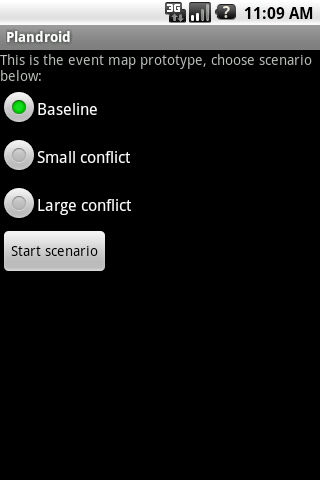
\includegraphics[height=50mm]{scenario}
  \caption{The scenario selection screen}
  \label{fig:scenario}
\end{figure}

In the prototype the user can go through the event creation procedure and handle
conflicts in different ways, supporting two different conflict types, major and
minor.

The event creation screen, shown in Figure \ref{fig:creation}, is not fully
featured in any way, only allowing the user to input the minimum amount of
information required to create an event. This was done so the user would focus
less on critiquing the actual screen, and more on the actual procedure of
inviting and handling schedule conflicts.

\begin{figure}[htb]
  \centering
  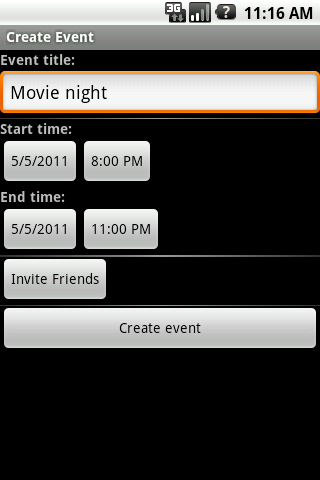
\includegraphics[height=50mm]{eventcreation}
  \caption{The event creation screen}
  \label{fig:creation}
\end{figure}

This screen also allows the user to invite friends by clicking on the
appropriate button, which pops up the screen shown in Figure
\ref{fig:invitation}, allowing the user to select which of their friends to
invite. The list is a standard Android ListView with an invite button at the
bottom, which the user has to scroll down to find.

\begin{figure}[htb]
  \centering
  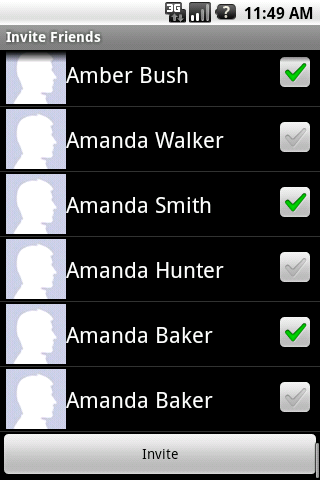
\includegraphics[height=50mm]{invitation}
  \caption{The invitation screen}
  \label{fig:invitation}
\end{figure}

The friends available in the prototype were randomly generated from a preset
list of names when the application is first launched, to give the user some data
to work with without requiring a lengthy input session beforehand.

When the user is done inviting friends, and click the invite button, they are
taken back to the event creation screen with their invited friends in a list, as
shown in Figure \ref{fig:invited}.

\begin{figure}[htb]
  \centering
  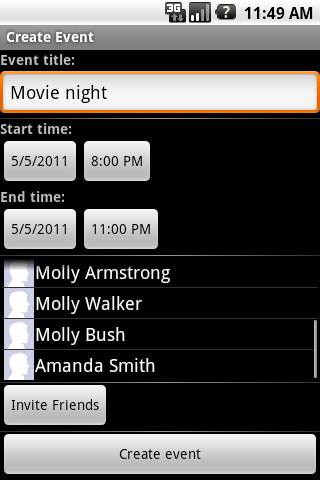
\includegraphics[height=50mm]{invited}
  \caption{Invited friends}
  \label{fig:invited}
\end{figure}

When the user then presses the button marked ``Create event'' and there are no
conflicts, a notification pops up saying that the event has been created and the
user is taken back to the scenario selection screen.

If there are conflicts (as is the case with the two last scenarios on the list),
then one of two dialogs can pop up. For a minor conflict (defined as 20\% of the
invited guests) the dialog in Figure \ref{fig:minor} pops up, allowing the user
to either ignore the warning or review the conflicts.

\begin{figure}[htb]
  \centering
  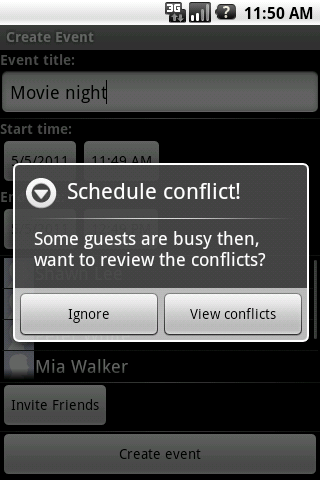
\includegraphics[height=50mm]{minor}
  \caption{The minor conflict dialog}
  \label{fig:minor}
\end{figure}

For a major conflict (defined as 60\% of the invited guests) the dialog in
Figure \ref{fig:major} pops up, prompting the user to reschedule the event, or
review the conflicts.

\begin{figure}[htb]
  \centering
  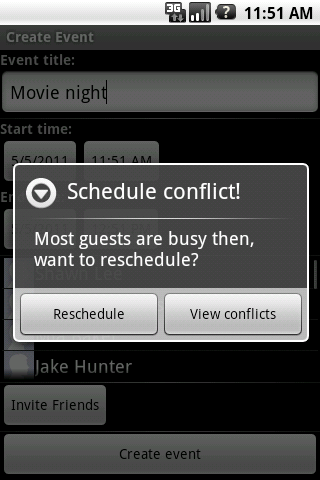
\includegraphics[height=50mm]{major}
  \caption{The major conflict dialog}
  \label{fig:major}
\end{figure}

Both of these dialogs give the user access to the screen in Figure
\ref{fig:resolve} for reviewing conflicts. On this screen, the user can see who
has schedule conflicts, what event is the cause of the conflict, and has the
option of removing them from the invite list.

The events listed under the conflicting users are chosen randomly from a
predefined list at the time of showing the conflicts, to give a little
randomness to every test.

\begin{figure}[htb]
  \centering
  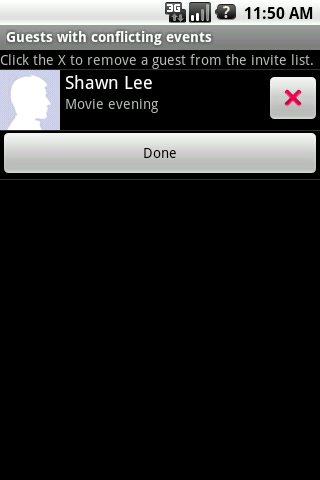
\includegraphics[height=50mm]{resolution}
  \caption{The conflict resolution screen}
  \label{fig:resolve}
\end{figure}

When the user chooses to reschedule the event from the major conflict dialog,
the application takes the user back to the event creation screen. The time and
date selectors are now highlighted, as in Figure \ref{fig:reschedule}.

\begin{figure}[htb]
  \centering
  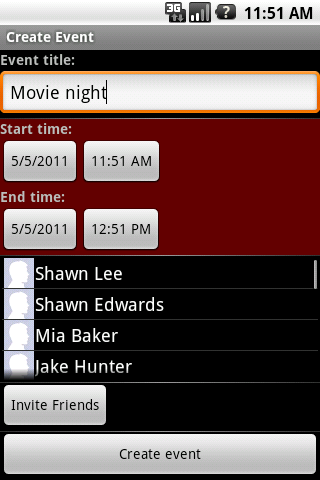
\includegraphics[height=50mm]{reschedule}
  \caption{The reschedule highlight}
  \label{fig:reschedule}
\end{figure}

When the user clicks the create event button again (regardless of whether the
time/date is changed or not) the event will then be created successfully,
another simplification done during the creation of the prototype.

\section{Final evaluation results}

Running the prototype through user tests proved enlightening. They showed that the
basic idea was sound, but the interface of the prototype was perhaps too
simplistic and fragmented.

The interface for inviting friends proved confusing, as the users weren't aware
of the Invite button at the end of the list to begin with, and there was no menu
option that performed the same function. They would either discover it by
accident while scrolling through the list, or have to be told where it was
located.

When it came to discovering and handling conflicts, the users agreed that the
functionality was promising, but lacking implementation-wise. A common problem
was for the user to remember state between the event creation and conflict
resolution screens. They would forget what time the event was set, and had to go
back and forth between the conflict resolution screen and the event information,
which in the prototype is an arduous task. There was also indication that the
choice of what to do during a schedule conflict is not obvious before the user
knows who is on the conflict list.

Most of the users found the conflict resolution screen easy to use and
understand, but a bit under-featured, although some felt that the red X buttons
were not immediately understandable, and pulled attention away from the
descriptive text. In addition, some of the users wanted access to more actions
than just removing from the guest list. All of the users agreed that showing the
guests' events was helpful in deciding what to do with a conflict, but almost
all agreed that showing the time as well would be even more helpful.

Users lamented the fact the system wasn't smarter, and proposed that perhaps the
system could first try automatically resolving the conflict, particularly in
minor ones, and propose suitable times for rescheduling, or automatically mark
certain guests as ``points of interest'' and give recommendations when resolving
conflicts.

In addition, some of the users showed concerns with the threshold values set for
minor and major conflicts, and wished that they were configurable, and the idea
of prioritizing friends so that certain friends were more important when
considering if a conflict is worth reporting was brought up. This point was also
brought up in similar research\cite{benhassine07,haynes97:_autom_meetin_sched_system}.

In summary, the interface as created in this prototype was workable, but could
do with some streamlining. The current flow hides crucial information behind a
dialog, and doesn't allow the user to go back and forth easily (as the dialog
will pop back up every time). In addition, the system is not as automated as it
could be, but it is a step in the right direction.

\chapter{Discussion}

\section{Success(es)}

\section{Flaw(s)}

\section{What did I learn}

\section{What would I do different}

\section{Next steps - future work}

In handheld and ubiquitous computing, a user's context is very dynamic. When
using applications in these settings, a user has much to gain by the effective
use of implicitly sensed context\cite{dey99:towar}.

\section{Conclusion}

\bibliography{report}{}
\bibliographystyle{plain}


\chapter{Appendices}

Will be provided as separate tex documents and put afterwards, these headers are
just for reminders

\section{Transcripts}

\section{Requirement documents}

\end{document}
